\addtocontents{toc}{\setcounter{tocdepth}{3}}
\chapter{Differentiation}
\section{What Is Differentiation?}

\textbf{None of this section on what differentiation has to be known for the exam (except for the notation), though it's incredibly useful to know.}

\subsection{Understanding Rate of Change}
To measure how much something has changed, the difference can be found. For example, look at the following graph of the EUR/USD price from January to December 2019.

\begin{figure}[h!]
	\centering
	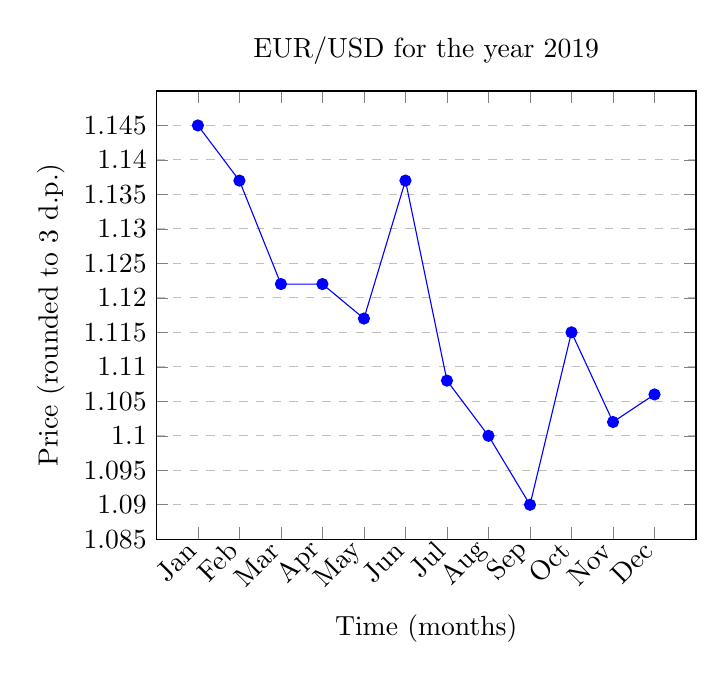
\begin{tikzpicture}
	\begin{axis}
	[
		title={EUR/USD for the year 2019},
		xlabel={Time (months)},
		ylabel={Price (rounded to 3 d.p.)},
		xmin=0,
		xmax=13,
		xtick={0,1,...,12},
		xticklabels={ ,Jan, Feb, Mar, Apr, May, Jun, Jul, Aug, Sep, Oct, Nov, Dec},
		ymin=1.085,
		ymax=1.150,
		ytick={1.085,1.090,...,1.145},
		x tick label style= {rotate=45, anchor=east},
		ymajorgrids=true,
		grid style=dashed,
		/pgf/number format/precision=3,
	]
		\addplot
		[
			color=blue,
			mark=*,
		] coordinates
		{
			(1,1.145) (2,1.137) (3,1.122) (4,1.122) (5,1.117) (6,1.137) (7,1.108) (8,1.100) (9,1.090) (10,1.115) (11,1.102) (12,1.106)
		};
	\end{axis}
	\end{tikzpicture}
	\caption{The EUR/USD course for January to December in 2019, rounded to 3 decimal places.}
	\label{fig:EURUSD}
\end{figure}

The change of the graph between December and January is the difference in their values. The exact values of those months are $1.145$ and $1.106$, so
\begin{align*}
	\text{difference in price} &= 1.145 - 1.106\\
	&=0.039\text{.}
\end{align*}

The rate of change is how quickly something changes, or in other words, the change that is experienced over time. The rate of change between January and December would be found by dividing the change by the time taken.

\begin{align*}
	\frac{\text{difference in price}}{\text{difference in time}} &=\frac{1.145-1.106}{12-1}\\[0.75em]
	&=\frac{0.039}{11} \approx 3.55\times10^{-3}
\end{align*}

More generally, the rate of change between any $x$ and $y$ is the difference in $y$ over the difference in $x$.
\begin{align*}
\text{rate of change} &= \frac{\text{difference in $y$}}{\text{difference in $x$}}
\end{align*}

\subsection{Paradox of the Instantaneous Rate of Change}
Suppose we would graph the distance over time of a quick vehicle. For reasons that'll become more clear later on, the symbol $s$ is used for displacement instead of distance. This graph just so happens to be the graph of $d=t^2$, how convenient!

\begin{figure}[h!]
	\centering
	\begin{tikzpicture}
		\begin{axis}
		[
			restrict y to domain=0:25,
			restrict x to domain=0:5,
			xlabel=$t (s)$,
			ylabel=$d (m)$,
			xmin=0,
			xmax=5,
			xtick={0,1,...,4},
			ymin=0,
			ymax=17,
			ytick={0,2,...,16},
			axis lines=center,
			smooth,
			samples=50
		]
		\addplot [color=black,mark=none] {x^2};
		\end{axis}
	\end{tikzpicture}
	\caption{Displacement ($s$) in metres over time ($t$) in seconds.}
	\label{POIexample}
\end{figure}

The vehicle starts slowly and quickly begins to travel faster and faster. It would be very helpful to know how quick the car is going at a time of, say, 3 seconds. In other words, it would be helpful to know its instantaneous rate of change at 3 seconds (remember, rate of change is the change in value over time, in this case it's the change in displacement over time, the velocity).

The problem is that there is no such thing as "instantaneous" rate of change. To have a rate of change, there must be a time that has elapsed. That's not very helpful though, there must be a way to find out how quick the car is going --- its velocity (symbol $v$) --- at in a moment in time.

The solution to this is to decrease the change in time that's being used until it's nearly $0$, as close to $0$ as you could get. By coming closer and closer to 0, a certain value is approached. Let's try using a change in time of 3.1 and 3.01 and see what happens.

\begin{align*}
	v&=\frac{\text{difference in $d$}}{\text{difference in $t$}} & v&=\frac{\text{difference in $d$}}{\text{difference in $t$}}\\[0.75em]
	v &= \frac{9.61-9}{3.1-3} & v &= \frac{9.0601-9}{3.01-3}\\
	&= 6.1 & &= 6.01
\end{align*}

As you can see, a value of $6$ is approached whenever a smaller value for the change in time is taken. As previously said, there is no such thing as instantaneous change, but instead the best approximation can be calculated. In this case, the best approximation for the rate of change can be concluded to be $6$.

That is what the derivative is. The best approximation for the rate of change.

Whenever the difference in the values will approach $0$, the symbol $d$ can be used, so more generally you can write for any $x$ and $y$,
\begin{equation}
	\text{derivative} = \frac{dy}{dx}\text{.}
\end{equation}

\subsection{Notation}
When an equation (such as $d=t^2$ like above) is differentiated, it is done with respect to one variable. Usually, equations are in the form $y=x$ where there might be lots on the $x$ side, but little on the $y$ side. When such an equation is differentiated, it is said to have been done ``with respect to x". The above example was differentiated with respect to $t$.

There are numerous ways of writing the derivative, each having a good use in different fields. In maths, two ways of writing the derivative are used: the one used by Leibniz, one of the independent discoverers of calculus, and the one used by Lagrange.

\subsubsection{Leibniz's Notation}
Leibniz notation is actually the one that has been used so far. The derivative of two variables $x$ and $y$ can be written as $\frac{dy}{dx}$ and is read out ``the derivative of $y$ with respect to $x$.
\subsection{Lagrange's Notation}
However, sometimes a function has to be differentiated. For example, the derivative of $f(x) = 6x^3$ is $18x^2$, but how is that written? A prime mark is added between the $f$ and $x$, and it is read as ``the derivative evaluated at $x$".
\begin{align*}
	f(x) &= 6x^3\\
	f'(x) &= 18x^2
\end{align*}


\section{A Shortcut to Differentiate}
Doing the above is very tedious, so luckily there is a shortcut that can be taken! Multiply the coefficient of the variable by the power, and subtract $1$ from the power. More formally,
\begin{align*}
	f(x) &= x^n\\
	f'(x) &= nx^{n-1}
\end{align*}

This is called the ``power rule".

\subsection{Examples}
Note that it's not required to continue to simplify after the derivative is found, however it might be helpful in more complex questions.

\begin{enumerate}
	\item
	\begin{align*}
		f(x) &= 5x^5\\
		f'(x) &= 25x^4
	\end{align*}
	\item
	\begin{align*}
		f(x) &= \frac{2}{x}\\
		&= x^{-2}\\
		f'(x) &= -2x^{-3}\\
		&= \frac{-2}{x^3}
	\end{align*}
	\item 
	\begin{align*}
		f(x) &= \frac{3}{\sqrt[4]{x^2}}\\
		&= \frac{3}{x^{\frac{2}{4}}}\\
		&= 3x^{-\frac{2}{4}}\\
		f'(x) &= -\frac{14}{4}x^{-\frac{6}{4}}\\[0.5em]
		&= \frac{-\frac{14}{4}}{x^{\frac{6}{4}}}\\[0.5em]
		&= \frac{-\frac{14}{4}}{\sqrt[4]{x^6}}
	\end{align*}
\end{enumerate}